\documentclass[aspectratio=1610, t]{beamer}\usepackage[]{graphicx}\usepackage[]{color}
% maxwidth is the original width if it is less than linewidth
% otherwise use linewidth (to make sure the graphics do not exceed the margin)
\makeatletter
\def\maxwidth{ %
  \ifdim\Gin@nat@width>\linewidth
    \linewidth
  \else
    \Gin@nat@width
  \fi
}
\makeatother

\definecolor{fgcolor}{rgb}{0.345, 0.345, 0.345}
\newcommand{\hlnum}[1]{\textcolor[rgb]{0.686,0.059,0.569}{#1}}%
\newcommand{\hlstr}[1]{\textcolor[rgb]{0.192,0.494,0.8}{#1}}%
\newcommand{\hlcom}[1]{\textcolor[rgb]{0.678,0.584,0.686}{\textit{#1}}}%
\newcommand{\hlopt}[1]{\textcolor[rgb]{0,0,0}{#1}}%
\newcommand{\hlstd}[1]{\textcolor[rgb]{0.345,0.345,0.345}{#1}}%
\newcommand{\hlkwa}[1]{\textcolor[rgb]{0.161,0.373,0.58}{\textbf{#1}}}%
\newcommand{\hlkwb}[1]{\textcolor[rgb]{0.69,0.353,0.396}{#1}}%
\newcommand{\hlkwc}[1]{\textcolor[rgb]{0.333,0.667,0.333}{#1}}%
\newcommand{\hlkwd}[1]{\textcolor[rgb]{0.737,0.353,0.396}{\textbf{#1}}}%
\let\hlipl\hlkwb

\usepackage{framed}
\makeatletter
\newenvironment{kframe}{%
 \def\at@end@of@kframe{}%
 \ifinner\ifhmode%
  \def\at@end@of@kframe{\end{minipage}}%
  \begin{minipage}{\columnwidth}%
 \fi\fi%
 \def\FrameCommand##1{\hskip\@totalleftmargin \hskip-\fboxsep
 \colorbox{shadecolor}{##1}\hskip-\fboxsep
     % There is no \\@totalrightmargin, so:
     \hskip-\linewidth \hskip-\@totalleftmargin \hskip\columnwidth}%
 \MakeFramed {\advance\hsize-\width
   \@totalleftmargin\z@ \linewidth\hsize
   \@setminipage}}%
 {\par\unskip\endMakeFramed%
 \at@end@of@kframe}
\makeatother

\definecolor{shadecolor}{rgb}{.97, .97, .97}
\definecolor{messagecolor}{rgb}{0, 0, 0}
\definecolor{warningcolor}{rgb}{1, 0, 1}
\definecolor{errorcolor}{rgb}{1, 0, 0}
\newenvironment{knitrout}{}{} % an empty environment to be redefined in TeX

\usepackage{alltt}


\usepackage{pgfplots}
\usepackage{amssymb}
\usepackage{amsmath}
\usepackage{pdfpages}

\makeatletter
\def\BState{\State\hskip-\ALG@thistlm}
\makeatother


\pgfplotsset{compat=1.15}

\def \A {\mathcal A}
\def \C {\mathcal C}
\def \E {\mathcal E}
\def \F {\mathcal F}
\def \G {\mathcal G}
\def \H {\mathcal H}
\def \M {\mathcal M}
\def \N {\mathcal N}
\def \cP {\mathcal P}
\def \S {\mathcal S}
\def \V {\mathcal V}

\def \P {\mathbf P}
\def \Q {\mathbf Q}
\def \I {{\mathbf 1}}

\def \R {\mathbb R}
\def \bF {\mathbb F}
\def \bG {\mathbb G}
\def \bH {\mathbb H}
\def \bE {\mathbb E}
\def \bN {\mathbb N}

\newcommand{\ud}{\mathrm d}
\newcommand{\ds}{\displaystyle}
%\newcommand{\esp}[2][\mathbb E] {#1\left[#2\right]}
\newcommand{\esp}[1]{\mathbb{E}^\Q \left[#1\right]}
\newcommand{\widehatesp}[2][\widehat{\mathbb E}] {#1\left[#2\right]}
%\newcommand{\var}[2][{\rm Var}] {#1\left(#2\right)}
\newcommand{\espp}[2][\mathbb {\widehat E}] {#1\left[#2\right]}
\newcommand{\condesp}[2][\G_t]       {\mathbb E\left.\left[#2\right|#1\right]}
\newcommand{\condespf}[2][\F_t]       {\mathbb E\left.\left[#2\right|#1\right]}
\newcommand{\condespfo}[2][\F_0]       {\mathbb E\left.\left[#2\right|#1\right]}
\newcommand{\condespfto}[2][\F_{t_0}]       {\mathbb E\left.\left[#2\right|#1\right]}
\newcommand{\condesphto}[2][\H_{t_0}]       {\mathbb E\left.\left[#2\right|#1\right]}
\newcommand{\condesph}[2][\H_t]       {\mathbb E\left.\left[#2\right|#1\right]}
\newcommand{\condespHH}[2][\H_t]       {\mathbb E^{\mathbf P^*}\left.\left[#2\right|#1\right]}
\newcommand{\condespho}[2][\H_{0}]       {\mathbb E\left.\left[#2\right|#1\right]}
\newcommand{\condesphoo}[2][\H_{0}]       {\mathbb E^{\mathbf P^*}\left.\left[#2\right|#1\right]}
\newcommand{\condesphu}[2][\H_{u}]    {\mathbb E \left.\left[#2\right|#1\right]}
\newcommand{\condesphT}[2][\H_{T}] {\mathbb E \left.\left[#2\right|#1\right]}
\newcommand{\condesphTT}[2][\H_{T}] {\mathbb E^{\mathbf P^*} \left.\left[#2\right|#1\right]}
%\newcommand{\condespff}[2][\F_{\tau-}]       {\widehat E\left.\left[#2\right|#1\right]}
%\newcommand{\condespg}[2][\G_\tau]       {\widehat E\left.\left[#2\right|#1\right]}
%\newcommand{\condespgg}[2][\G_{\tau-}]       {\widehat E\left.\left[#2\right|#1\right]}
\newcommand{\doleans}[1] {\mathcal E\left(#1\right)}
%\newcommand{\ind}{\mbox{1 \hspace{-10 pt} I}}
\newcommand{\condesphh}[2][\H_{\tau-}]   {\mathbb E\left.\left[#2\right|#1\right]}
\newcommand{\CL}{\operatorname{CL}}
\newcommand{\CVA}{\operatorname{CVA}}
\newcommand{\CDS}{\operatorname{CDS}}
%%%%%%%%%%%%%%%%%%%%%%%%%%%%%%%%%
%% ====== Define Style ======= %% 
%%%%%%%%%%%%%%%%%%%%%%%%%%%%%%%%%

%% ====== title page ======

	%% required inputs
	\author{Sourav Adhikari, {Verena K\"ock}}             %% Author
	\title{\LARGE {Classification Methods: \\ Applications in R} }  %% Presentation Title
	\newcommand{\titleLength}{2}         %% Title length: 2 = 2 lines, 1 = 1 line
	\date{Date: 2022-06-13}                    %% Date, leave blank to avoid include, comment out to get current dat
	\newcommand{\titleBackground}{3}     %% Background graphic: 0 = none, 1 = D2, 2 = Campus, 3 = Forum

	%% optional inputs 
	\subtitle{ }                          %% (optional) Subtitle, comment out lines to avoid include
	\newcommand{\affiliationText}{\textit{ Project Presentation - ADAR}} %% (optional) Title page text, comment out lines to avoid include, enlarges white box on tile page

%% ====== footer ======
	\newcommand{\placementLogoFooter}{1}           %% 1 = logo right, 2 = logo left
	\newcommand{\slideNumberLabelFooter}{Slide}    %% Page/Slide/Folie/Seite
	\newcommand{\dateFooter}{2022-06-13}           %% (optional) Date in footline, comment out lines to avoid include
	\newcommand{\textFooter}{} %% (optional) Text for footline, e.g. title, comment out lines to avoid include, max. 1 line

%% ====== header (optional) ====== 
	%\newcommand{\sectionHeader}{Section (optional)}  %% (optional) Text before section number, e.g. Section or Kapitel; comment out to omit in presentation

%% ====== end page (optional) ====== 
	%\newcommand{\address}{Add address here \\ (optional)}   %% (optional) Address text for end page, comment out lines to avoid include and to avoid end page


%%%%%%%%%%%%%%%%%%%%%%%%%%%%%
%% ====== Preamble ======= %% 
%%%%%%%%%%%%%%%%%%%%%%%%%%%%%

%% ====== settings (optional) ======
	\usenavigationsymbolstemplate{}             %% (optional) Comment out to include navigation bar
	%\newcommand{%\includeTocAtBeginSection}{}   %% (optional) Table of contents at begin of every section, comment out lines to avoid include
	%\newcommand{%\includePartPages}{}
	%\newcommand{%\includeTocAtBeginPart}{}

%% ====== load beamer style ======
	\usepackage{beamerthemewu2017}


%%%%%%%%%%%%%%%%%%%%%%%%%%%%%%%%%%%
%% ====== Begin Document ======= %% 
%%%%%%%%%%%%%%%%%%%%%%%%%%%%%%%%%%%

\IfFileExists{upquote.sty}{\usepackage{upquote}}{}
\begin{document}


%% ====== Title Page ======
\maketitle

													
%% ====== Outline at beginning of document ======
%\begin{frame}{Outline (optional)}
%		\tableofcontents							%% (optional) Table of contents, comment out lines to avoid include
%\end{frame}
													

%% ====== Section  ======
\section{Motivation}


%% ====== Slide ======
\begin{frame}{(Statistical) Classification: What is it?}

\begin{itemize}
\item The problem of identifying which of a set of categories an observation belongs to.
  \begin{itemize}
  \item E.g. assigning an incoming email to "spam" or "inbox" mailbox.
  \end{itemize}
\item Classification can be thought of as two separate problems: 
  \begin{itemize}
  \item binary classification 
  \item multiclass classification.
  \end{itemize}
\medskip
\item \textcolor{wublue}{\textbf{Examples}} for classification methods are:
  \begin{itemize}
  \item Naive Bayes
  \item k-Nearest Neighbors
  \item Neural Networks
  \item Others: Decision Trees, Random Forest, Logistic Regression, SVM, etc.
  \end{itemize}
  \medskip
\item  \textcolor{wublue}{\textbf{This project:}} We explain and present results from first three methods: Naive Bayes, k- Nearest Neighbors and Neural Networks.
\end{itemize}

\end{frame}

\section{Dataset1}
\begin{frame}{The IRIS dataset I}
\begin{itemize}
  \item The data contains 4 measurements for 150 flowers from each of three species of \textit{iris}:
    \begin{itemize}
    \item \texttt{{Sepal.Length}}, \texttt{Sepal.Width}, \texttt{Petal.Length} and \texttt{Petal.Width} in cm
    \item \texttt{Species}: setosa, virginica and versicolor
    \end{itemize}
\end{itemize}
    	\begin{tabular}{@{}c@{\hspace{.5cm}}c@{}}
		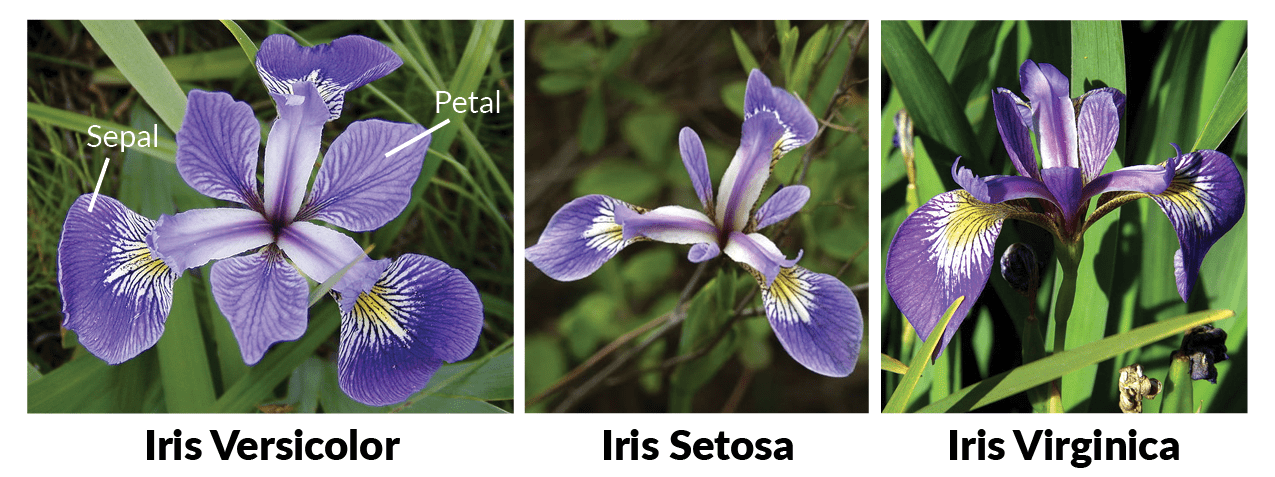
\includegraphics[width=0.95\textwidth]{iris.png}
	\end{tabular}
\end{frame}
   
\section{Dataset2}
\begin{frame}{IRIS Data: \small setosa(red), versicolor(gr.), virginica(bl.)}
\vspace{-1.9cm}
\begin{knitrout}
\definecolor{shadecolor}{rgb}{0.969, 0.969, 0.969}\color{fgcolor}

{\centering 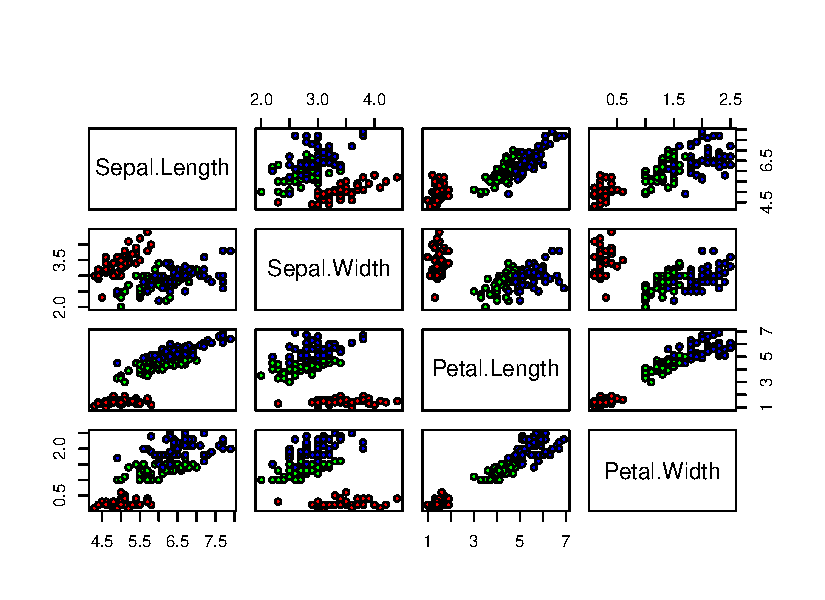
\includegraphics[width=\maxwidth]{figure/scatterplot-1} 

}


\end{knitrout}
\end{frame}


\begin{frame}[t]{Validation of the training procedure} \small
  \begin{itemize}
    \item We split the data into training (points) and testing set (squares) in the ratio 67:33.
    \item We perform k-fold cross validation.
   \end{itemize}

   \vspace{-1.8cm}
   





\begin{knitrout}
\definecolor{shadecolor}{rgb}{0.969, 0.969, 0.969}\color{fgcolor}

{\centering 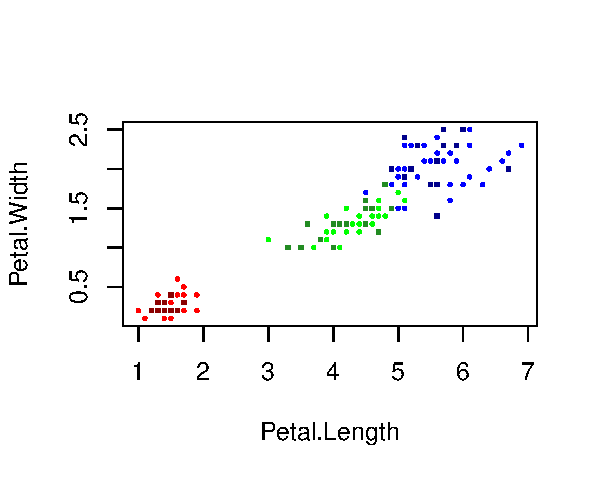
\includegraphics[width=\maxwidth]{figure/plot-1} 

}


\end{knitrout}

\end{frame}

\begin{frame}{Naive Bayes}
\begin{itemize}
\item Naive Bayes classifiers are simple "probabilistic classifiers" based on Bayes' theorem.
\item \textit{Disadvantage}: (\textbf{Strong}) assumption, that the features are independent (i.e presence of one particular feature does not affect the other). Hence the adjective \textbf{naive}.
\item \textit{Advantage}: Requires only a small number of training data to estimate the parameters.
\item Let $y$ be the category variable, and $X$ the features, then \textcolor{wublue}{\textbf{Bayes theorem}} is:
$$P(y|X) = \frac{P(X|y)P(y)}{P(X)},$$

\item \textcolor{wublue}{\textbf{Steps:}}
\begin{enumerate}\small
  \item Estimate prior probability $P(X)$: Compute the relative frequency of each class/species.
  \item Assume normal distribution for each class (species). Estimate $\mu$ and $\sigma^2$ for each class.
  \item For a new observation, apply Bayes theorem (and normalize) to get a vector of probabilities, e.g. $(\bf{0.5},0.25,0.25)$!
\end{enumerate}
\end{itemize}
\end{frame}

\begin{frame} {Naive Bayes in R} 

\vspace{-2cm}

\begin{knitrout}
\definecolor{shadecolor}{rgb}{0.969, 0.969, 0.969}\color{fgcolor}

{\centering 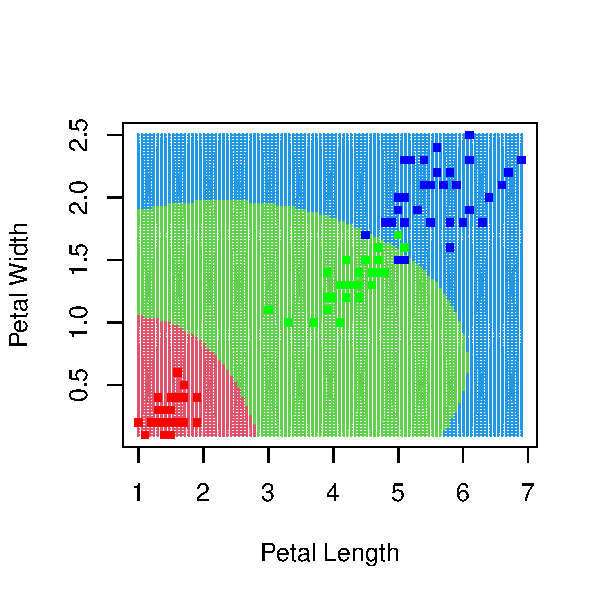
\includegraphics[width=\maxwidth]{figure/nb1-1} 

}


\end{knitrout}

\end{frame}

\begin{frame}{K-nearest neighbors}
\begin{itemize}
\item A non-parametric supervised learning method

\item Uses a distance metric to make classifications or predictions about the grouping of an individual data point.

\item Object is assigned to the class it is most common with among its k nearest neighbors.

\item \textit{Advantages}: Easy to understand and implement, no assumptions required
\item \textit{Disadvantages}: Curse of Dimensionality
\end{itemize}


\end{frame}

\begin{frame}{1-nearest neighbour}
\vspace{-2cm}
\begin{knitrout}
\definecolor{shadecolor}{rgb}{0.969, 0.969, 0.969}\color{fgcolor}

{\centering 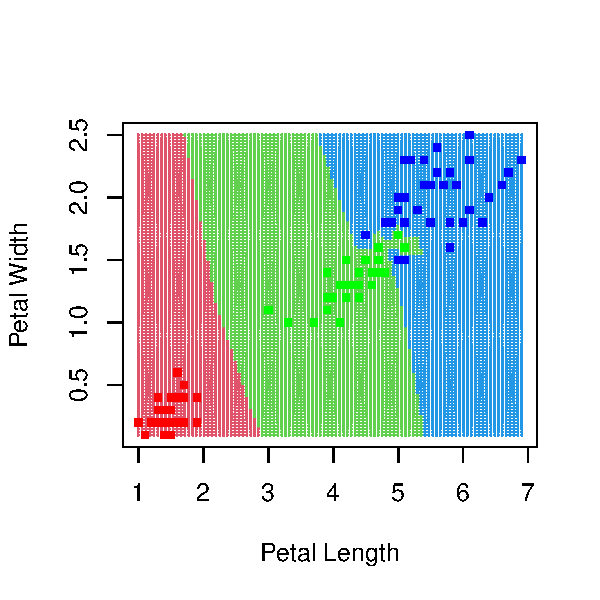
\includegraphics[width=\maxwidth]{figure/knn1-1} 

}


\end{knitrout}
\end{frame}



%% ====== Slide ======
\begin{frame}[t]{Neural Networks}

\begin{itemize}
  \item Neural networks (NNs) are computing systems inspired by the biological neural networks that constitute animal brain. 
  \item They learn forming probability-weighted associations between ``input" and ``result". 
\end{itemize}

\centering
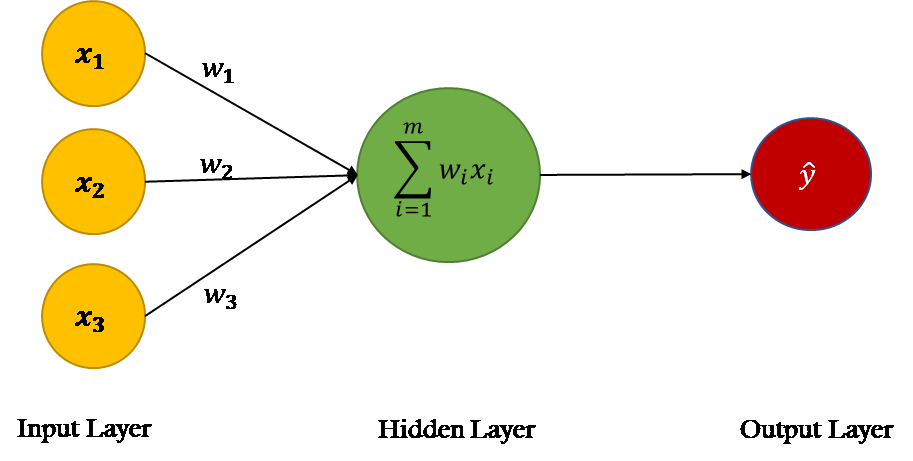
\includegraphics[scale=0.3]{neuron.png}
        
\end{frame}


%% ====== Slide ======
\begin{frame}[t]{Neural Networks}

\begin{itemize}
  \item For classification tasks, NNs utilize an activation function, for example a logistic function:
	$$f(x) = \frac{L}{1 + e^{-k(x - x_0)}}$$
  
\end{itemize}

\centering
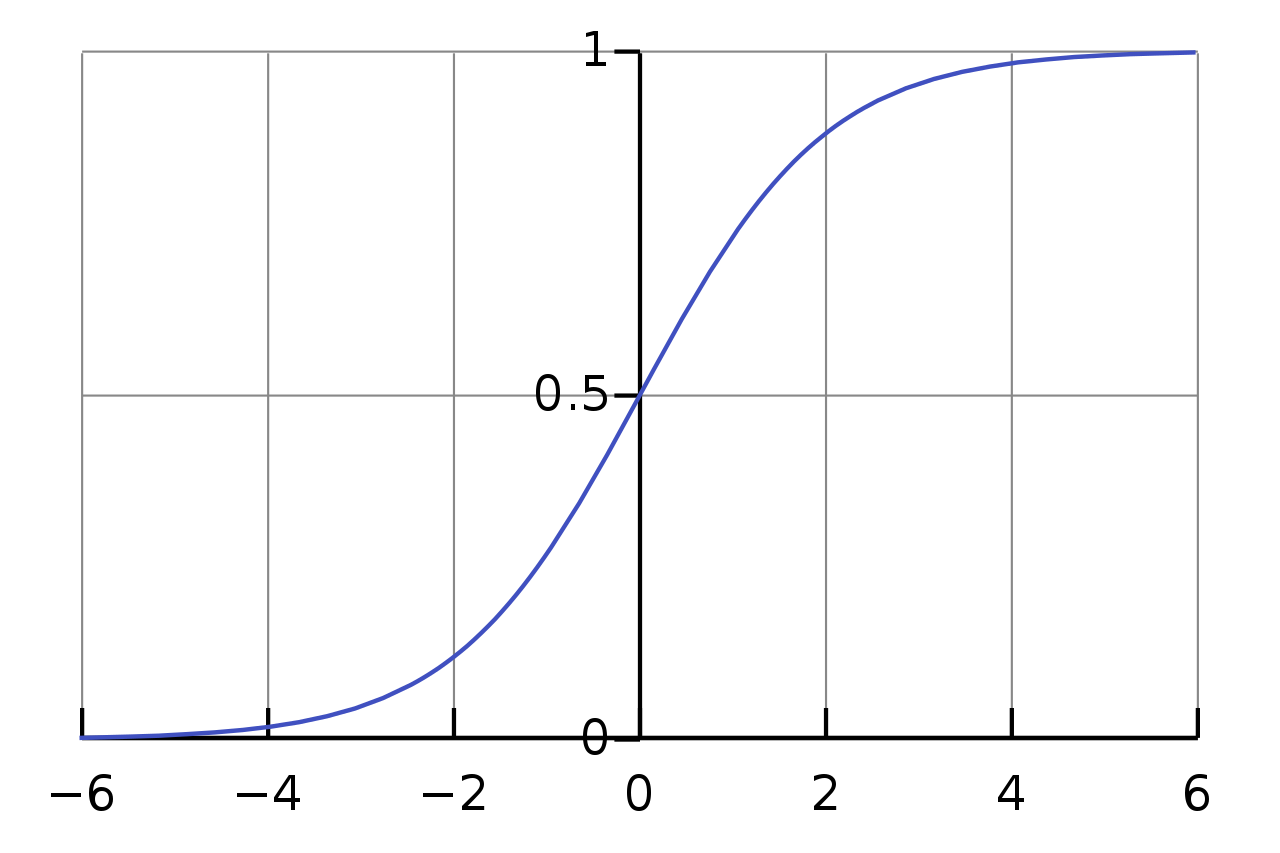
\includegraphics[scale=0.17]{logistic.png}
        
\end{frame}

\begin{frame}{Neural network}

\vspace{-2cm}


\begin{knitrout}
\definecolor{shadecolor}{rgb}{0.969, 0.969, 0.969}\color{fgcolor}

{\centering 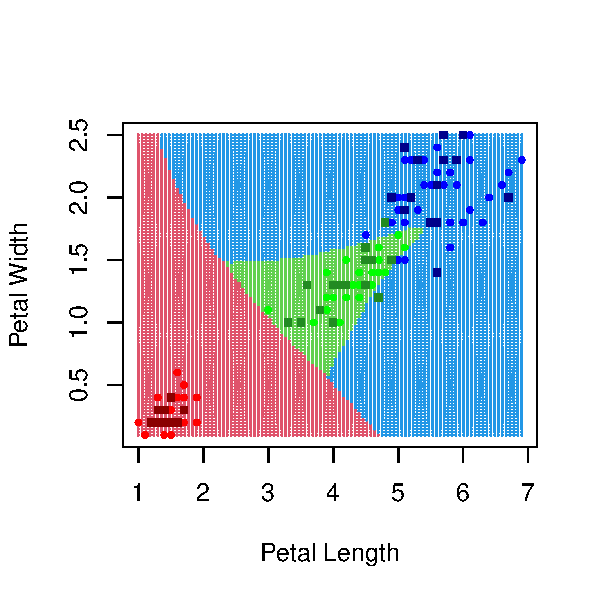
\includegraphics[width=\maxwidth]{figure/nnw1-1} 

}


\end{knitrout}

\end{frame}

%% ====== Slide ======
%\begin{frame}[t]{Neural Networks}

%\centering
%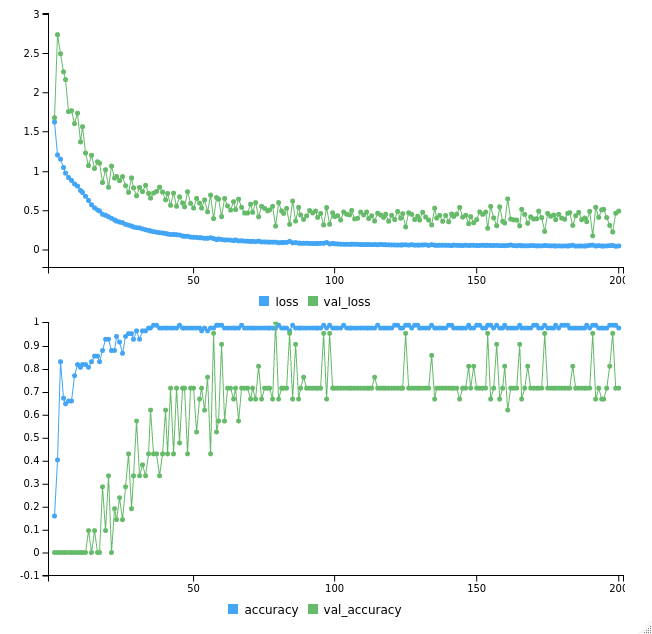
\includegraphics[scale=0.5]{nn_learn.png}
        
%\end{frame}




%% ====== Slide ======
\begin{frame}[t]{Cross Validation}

\begin{itemize}
  \item A resampling procedure for model validation.
  \item Assessing how the results of a statistical analysis will generalize to an independent data set.
  \item Estimates how accurately a predictive model will perform in practice.
  \item For the Iris dataset, we specifically perform the k-fold cross validation.
  
\end{itemize}
        
\end{frame}

%% ====== Slide ======
\begin{frame}[t]{k-fold Cross Validation}

\begin{itemize}
  \item Shuffle the dataset randomly.
  \item Split the dataset into k groups.
  \item For each unique group:
  \begin{itemize}
    \item Take the group as a hold out or test data set.
    \item Take the remaining groups as a training data set.
    \item Fit a model on the training set and evaluate it on the test set.
    \item Retain the evaluation score and discard the model.
  \end{itemize}
  \item Summarize the skill of the model using the sample of model evaluation scores.
  \item Note: The k value must be chosen carefully for the data sample.
\end{itemize}
        
\end{frame}

%% ====== Slide ======
\begin{frame}[t]{k-fold Cross Validation}

\begin{itemize}
  \item Performed using the function \texttt{train()} included in the R package \texttt{caret}.
  
\begin{knitrout}\scriptsize
\definecolor{shadecolor}{rgb}{0.969, 0.969, 0.969}\color{fgcolor}\begin{kframe}
\begin{alltt}
\hlkwd{library}\hlstd{(caret)}
\end{alltt}


{\ttfamily\noindent\itshape\color{messagecolor}{\#\# Lade nötiges Paket: ggplot2}}

{\ttfamily\noindent\itshape\color{messagecolor}{\#\# Lade nötiges Paket: lattice}}\begin{alltt}
\hlstd{tc} \hlkwb{<-} \hlkwd{trainControl}\hlstd{(}\hlkwc{method} \hlstd{=} \hlstr{"cv"}\hlstd{,} \hlkwc{number} \hlstd{=} \hlnum{10}\hlstd{)}

\hlstd{fit} \hlkwb{<-} \hlkwd{train}\hlstd{(Species} \hlopt{~}\hlstd{.,}\hlkwc{data} \hlstd{=} \hlkwd{data.frame}\hlstd{(iris.training,}\hlstr{"Species"}\hlstd{=}
              \hlstd{iris.trainingtarget),} \hlkwc{method} \hlstd{=} \hlstr{"nb"}\hlstd{,}\hlkwc{trControl} \hlstd{= tc,} \hlkwc{metric} \hlstd{=} \hlstr{"Accuracy"}\hlstd{)}
\end{alltt}
\end{kframe}
\end{knitrout}

  \item k=10 is used.
  \item Qualitative aspect is measured by Cohen's kappa score and the accuracy measure.  
  \item Measures the agreement between two raters who each classify N items into C mutually exclusive categories:
  
  $$\kappa = \frac{p_o - p_e}{1 - p_e}$$
\end{itemize}
        
\end{frame}





%% ====== Slide ======
\begin{frame}[fragile]{k-fold Cross Validation: Naive Bayes}

\begin{knitrout}\scriptsize
\definecolor{shadecolor}{rgb}{0.969, 0.969, 0.969}\color{fgcolor}\begin{kframe}
\begin{alltt}
\hlkwd{library}\hlstd{(caret)}
\hlkwd{set.seed}\hlstd{(}\hlnum{1}\hlstd{)}
\hlstd{tc} \hlkwb{<-} \hlkwd{trainControl}\hlstd{(}\hlkwc{method} \hlstd{=} \hlstr{"cv"}\hlstd{,} \hlkwc{number} \hlstd{=} \hlnum{10}\hlstd{)}
\hlstd{fit} \hlkwb{<-} \hlkwd{train}\hlstd{(Species} \hlopt{~}\hlstd{.,}\hlkwc{data} \hlstd{=} \hlkwd{data.frame}\hlstd{(iris.training,}\hlstr{"Species"}\hlstd{=}
  \hlstd{iris.trainingtarget),}\hlkwc{method} \hlstd{=} \hlstr{"nb"}\hlstd{,}\hlkwc{trControl} \hlstd{= tc,} \hlkwc{metric} \hlstd{=} \hlstr{"Accuracy"}\hlstd{)}
\hlstd{fit}\hlopt{$}\hlstd{results}
\end{alltt}
\begin{verbatim}
##   usekernel fL adjust  Accuracy     Kappa AccuracySD    KappaSD
## 1     FALSE  0      1 0.9607071 0.9403631  0.0510286 0.07750075
## 2      TRUE  0      1 0.9507071 0.9252115  0.0522565 0.07933520
\end{verbatim}
\begin{alltt}
\hlstd{pred} \hlkwb{<-} \hlkwd{predict}\hlstd{(fit, iris.test)}
\hlstd{result}\hlkwb{<-}\hlkwd{confusionMatrix}\hlstd{(iris.testtarget, pred)}
\hlkwd{sum}\hlstd{(}\hlkwd{diag}\hlstd{(result}\hlopt{$}\hlstd{table))}\hlopt{/}\hlkwd{sum}\hlstd{(result}\hlopt{$}\hlstd{table)}
\end{alltt}
\begin{verbatim}
## [1] 0.9574468
\end{verbatim}
\end{kframe}
\end{knitrout}

        
\end{frame}

%% ====== Slide ======

\begin{frame}[fragile]{k-fold Cross Validation: k-nearest Neighbours}
\begin{knitrout}\scriptsize
\definecolor{shadecolor}{rgb}{0.969, 0.969, 0.969}\color{fgcolor}\begin{kframe}
\begin{alltt}
\hlkwd{set.seed}\hlstd{(}\hlnum{1}\hlstd{)}
\hlstd{knn_fit} \hlkwb{<-} \hlkwd{train}\hlstd{(Species} \hlopt{~}\hlstd{.,}\hlkwc{data} \hlstd{=} \hlkwd{data.frame}\hlstd{(iris.training,}\hlstr{"Species"}\hlstd{=}
  \hlstd{iris.trainingtarget),} \hlkwc{method} \hlstd{=} \hlstr{"knn"}\hlstd{,} \hlkwc{trControl}\hlstd{=tc,} \hlkwc{metric} \hlstd{=} \hlstr{"Accuracy"}\hlstd{)}
\hlstd{knn_fit}\hlopt{$}\hlstd{results}
\end{alltt}
\begin{verbatim}
##   k  Accuracy     Kappa AccuracySD    KappaSD
## 1 5 0.9609091 0.9403883 0.05053433 0.07705315
## 2 7 0.9609091 0.9403883 0.05053433 0.07705315
## 3 9 0.9800000 0.9696970 0.04216370 0.06388440
\end{verbatim}
\begin{alltt}
\hlstd{pred} \hlkwb{<-} \hlkwd{predict}\hlstd{(knn_fit,iris.training)}
\hlstd{result}\hlkwb{<-}\hlkwd{confusionMatrix}\hlstd{(iris.trainingtarget, pred)}
\hlkwd{sum}\hlstd{(}\hlkwd{diag}\hlstd{(result}\hlopt{$}\hlstd{table))}\hlopt{/}\hlkwd{sum}\hlstd{(result}\hlopt{$}\hlstd{table)}
\end{alltt}
\begin{verbatim}
## [1] 0.9805825
\end{verbatim}
\end{kframe}
\end{knitrout}
\end{frame}


%% ====== Slide ======
\begin{frame}[fragile]{k-fold Cross Validation: Neural Network}

\begin{knitrout}\scriptsize
\definecolor{shadecolor}{rgb}{0.969, 0.969, 0.969}\color{fgcolor}\begin{kframe}
\begin{alltt}
\hlkwd{set.seed}\hlstd{(}\hlnum{1}\hlstd{)}
\hlstd{nnet_fit} \hlkwb{<-} \hlkwd{train}\hlstd{(Species} \hlopt{~}\hlstd{.,}\hlkwc{data} \hlstd{=} \hlkwd{data.frame}\hlstd{(iris.training,}\hlstr{"Species"}\hlstd{=}
  \hlstd{iris.trainingtarget),} \hlkwc{method} \hlstd{=} \hlstr{"nnet"}\hlstd{,} \hlkwc{trControl}\hlstd{=tc,} \hlkwc{metric} \hlstd{=} \hlstr{"Accuracy"}\hlstd{,}\hlkwc{trace} \hlstd{=} \hlnum{FALSE}\hlstd{)}
\hlstd{nnet_fit}\hlopt{$}\hlstd{results}
\end{alltt}
\begin{verbatim}
##   size decay  Accuracy     Kappa AccuracySD    KappaSD
## 1    1 0e+00 0.8212121 0.7208569 0.13431685 0.21313940
## 2    1 1e-04 0.7517172 0.5951669 0.26779376 0.44643182
## 3    1 1e-01 0.9497980 0.9223883 0.07103029 0.10906072
## 4    3 0e+00 0.9536364 0.9280673 0.08891242 0.13915422
## 5    3 1e-04 0.9618182 0.9419596 0.04938557 0.07510644
## 6    3 1e-01 0.9800000 0.9694639 0.04216370 0.06437816
## 7    5 0e+00 0.9309091 0.8930024 0.09459206 0.14926891
## 8    5 1e-04 0.9618182 0.9425365 0.04938557 0.07436975
## 9    5 1e-01 0.9800000 0.9694639 0.04216370 0.06437816
\end{verbatim}
\begin{alltt}
\hlstd{pred} \hlkwb{<-} \hlkwd{predict}\hlstd{(nnet_fit,iris.training); result}\hlkwb{<-}\hlkwd{confusionMatrix}\hlstd{(iris.trainingtarget, pred)}
\hlkwd{sum}\hlstd{(}\hlkwd{diag}\hlstd{(result}\hlopt{$}\hlstd{table))}\hlopt{/}\hlkwd{sum}\hlstd{(result}\hlopt{$}\hlstd{table)}
\end{alltt}
\begin{verbatim}
## [1] 0.9902913
\end{verbatim}
\end{kframe}
\end{knitrout}
        
\end{frame}

%% ====== Slide ======
\begin{frame}[t]{Summary}

\begin{center}
\begin{tabular}{ c c c }
 \textbf{Method} & \textbf{Accuracy Score}  & \textbf{Accuracy Test} \\
 Naive Bayes & 0.9607 &  0.9574 \\
 9-NN & 0.9800 & 0.9806 \\
 Neural Network & 0.9800  & 0.9903  
\end{tabular}

\begin{itemize}
  \item Among the methods discussed, kNN with k = 9 offers the highest rate of accuracy.
  \item There is no ``one method fits all" approach when undertaking classification tasks.
\end{itemize}
\end{center}
        
\end{frame}



%% ====== End Document ====== %%

\begin{frame}{References}
\begin{thebibliography}{10}
\setbeamertemplate{bibliography item}[text]
\bibitem{Md}
Gareth James, Daniela Witten, Trevor Hastie, Robert Tibshirani, "An Introduction to Statistical Learning : with Applications in R", Springer, 2013.
\bibitem{Md}
McCulloch, Warren, Walter Pitts, "A Logical Calculus of Ideas Immanent in Nervous Activity", Bulletin of Mathematical Biophysics. 5 (4): 115–133, 1943.

\end{thebibliography}

\end{frame}

%% ====== End Document ====== %%
\end{document}
